\documentclass[onecolumn]{article}
\usepackage{CJKutf8, graphicx}%导入CJKutf8包,并且激活中文、日文、韩文的uft8编码
\usepackage[utf8]{inputenc}

\title{短视频传输实验报告}
\author{计研173 \quad 陈雨兰 \quad 2017310787  \\ 计研173 \quad 蔡文静 \quad 2017210866}
\date{January 2018}

\begin{document}
\begin{CJK*}{UTF8}{gbsn}

\maketitle
\section{介绍}
该项目实现了从客户端到服务器端的短视频的快速上传。我们在UDP协议传输数据的基础上加上了数据解压缩、差错控制和数据包校验,实现了短视频的快速准确的传输。

\section{项目设计与分析}
\subsection{算法框架}
为了应对UDP传输中的丢包和乱序的情况,我们采用前向纠错技术进行丢包恢复。
该算法由发送方进行FEC编码引入冗余包,接收方进行FEC解码并恢复丢失的数据包。
对于包乱序和包重复,我们采用QOS乱序恢复处理,该QOS方案特点是在没有丢包的情况下,不引入任何系统延时,并且可以通过可控的丢包等待时延来适应不同的信道乱序程度。
QOS需要在接收端进行FEC解码前进行,确保送FEC解码模块的数据包序号是正确的(不存在乱序,仅存在丢包)。
图1为算法的主要框架。

\begin{figure}[h]
	\centering
	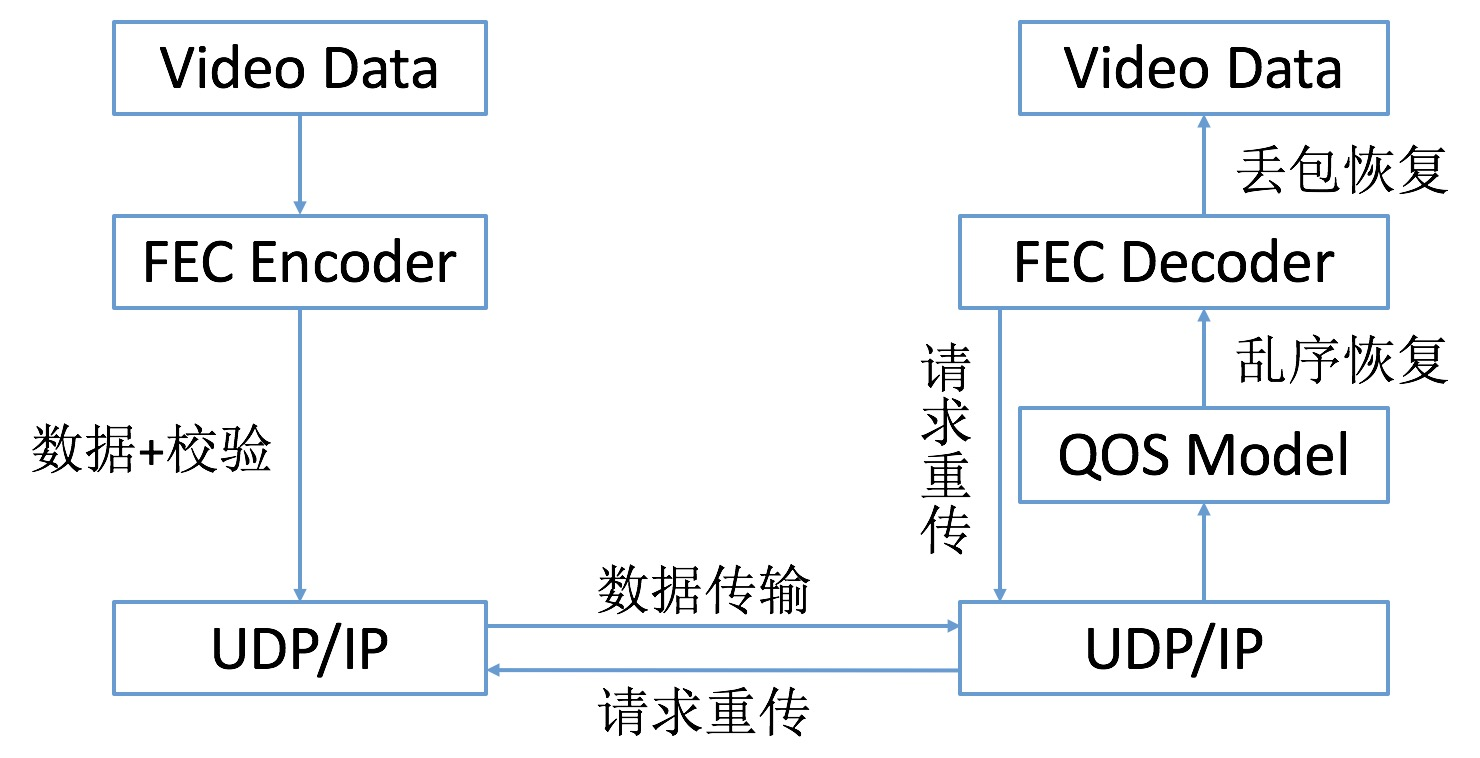
\includegraphics[width=4in]{frame.jpg}
	\caption{算法框架}
	\label{fig:frame}
\end{figure}

本算法侧重于优化具备随机信道特性的传输链路,即连续丢包的概率远低于单包丢失的情况。
当丢包率超过前向纠错的恢复上限时,算法无法恢复所有数据,此时若要保证传输的正确性,需要引入请求重传机制。

\subsection{传输协议}
TCP和UDP是比较常用的传输协议。TCP提供可靠的通信传输,而UDP则常被用于让广播和细节控制交给应用的通信传输。
\subsubsection{TCP协议}
TCP是一种面向连接的协议,能提供可靠的传输服务,即TCP通过检验和、序列号、确认应答、重发控制、连接管理以及窗口控制等机制实现可靠性传输。TCP充分实现了数据传输时各种控制功能,可以进行丢包的重发控制,还可以对次序乱掉的分包进行顺序控制。但是这些功能也限制了TCP数据传输的速度,而且使得系统资源要求较高。
\subsubsection{UDP协议}

UDP是一个非连接的协议,传输数据之前源端和终端不建立连接,当它想传送时就简单地去抓取来自应用程序的数据,并尽可能快地把它扔到网络上。在发送端,UDP传送数据的速度仅仅是受应用程序生成数据的速度、计算机的能力和传输带宽的限制;在接收端,UDP把每个消息段放在队列中,应用程序每次从队列中读一个消息段。由于传输数据不建立连接,因此也就不需要维护连接状态,包括收发状态等,因此一台服务机可同时向多个客户机传输相同的消息。UDP信息包的标题很短,只有8个字节,相对于TCP的20个字节信息包的额外开销很小。UDP使用尽最大努力交付,即不保证可靠交付,因此主机不需要维持复杂的链接状态表(这里面有许多参数)。UDP是面向报文的。发送方的UDP对应用程序交下来的报文,在添加首部后就向下交付给IP层。既不拆分,也不合并,而是保留这些报文的边界,因此,应用程序需要选择合适的报文大小。

基于上述分析,TCP和UDP分别有如下几个特点:
\begin{itemize}
\item TCP面向连接;UDP面向无连接
\item TCP面向字节流;UDP面向报文
\item TCP首部开销大,有20字节,且占用资源较多;UDP首部开销小,只有8字节,且占用资源少
\item TCP提供可靠的服务,即,通过TCP连接传送的数据,无差错,不丢失,不重复,且按序到达;UDP尽最大努力交付,即不保证可靠交付;
\item UDP发送数据速度更快
\end{itemize}

\subsection{丢包恢复}
\begin{figure}[h]
	\centering
	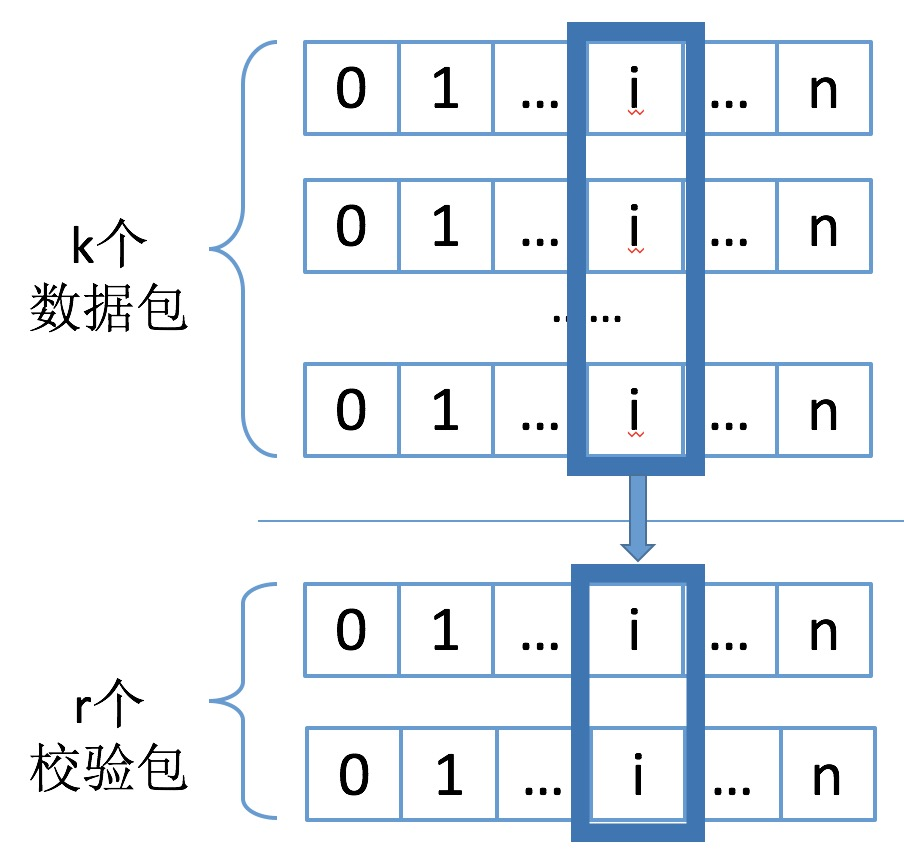
\includegraphics[width=2in]{FEC.jpg}
	\caption{前向纠错算法}
	\label{fig:FEC}
\end{figure}

前向纠错(FEC)技术近年来广泛应用于信息处理的各个领域。
FEC算法通过主动提高冗余度来降低丢包重传的频率,从而降低传输延时。

本次实验中的FEC算法在应用层实现,以数据包为单位进行丟包检测与丟包恢复。
UDP协议保障了包内数据的正确性,我们无需考虑包内纠错,只处理包丢失的情况。
每k 个数据包可以生成r个冗余包,共同构成一个组,即为一个独立的处理单元。
组内每个包拥有连续的编号,通过读取编号可以判断数据包的丟失情况,并予以恢复(冗余包丟失无需恢复)。 

由于冗余性的存在,一个组中任意k个包可以用来重建原始的k个数据包。
如果丟失数据包数小于或等于r,接收者收到一个Group中任意的k个数据包后,即可以通过组号信息确定丟失包的相对位置并进行FEC解码,恢复k个原始媒体包。
这里我们定义冗余包数r与原始媒体包数k的比值为FEC编码冗余度,冗余度越高,抗丟包能力越强,同时传输效率也越低。
找到传输效率与抗丟包能力二者的折中,从而 选择合适的冗余度配置是本方案实际应用过程中必须考虑的问题。

实验中采用Vandermonde矩阵RS算法,下面对算法进行简述:

 (1)数据包分割
 
对数据包进行FEC编码运算首先进行的是包内分割,将数据包分割为多个定长单元,定长单元称为字,设字长为wbits,w的取值一般为8、16、或者32。FEC编码对 k个原始媒体包逐字进行处理,生成m个冗余数据包中与之对应的字。例如现有两个 原始数据包Dl、D2,包的长度都为b bytes (对于包长不足b bytes的使用0补齐), 字长为wbits,那么一个数据包的总字长为l=8b/w。用这两个数据包产生两个冗余包 Cl、C2的过程简述如下:

(2) Vandermonde编解码以及改进

设k个原始数据包为$D= (D_1,D_2,\dots,D_k)$,r个冗余包为$C=(C_1,C_2,\dots,C_r)$,那么传输组可以表示为$Y= (D,C)$。
B 为rxk维FEC生成矩阵,则冗余包生成满足:

$$C=BD$$

在接收端,如果接收者收到了 Group中的任意k个数据包,即可根据所收到的数据包在组中的位置,从FEC生成矩阵B中提取对应的行, 组成一个新的kxk维矩阵B’,显然

$$7 =BD$$

如果B’为非奇异矩阵,那么就可以通过如下逆变换得到原始数据包,完成恢复。

$$D = (B)~1Y$$

设计RS码的关键在于怎样设计生成矩阵B,也就是其系数矩阵G。本方案使用Vandermonde矩阵来构建系数矩阵G。
常规定义Vandermonde矩阵V,r*k维,如下 所示:

%$V=\begin{bmatrix}
%1      & 1      & 1      & \cdots & 1       \\
%1      & 2      & 2^2    & \cdots & 2^{k-1} \\
%\vdots & \vdots & \vdots & \ddots & \vdots  \\
%1      & r      & r^2    & \cdots & r^{k-1}
%\end{bmatrix}$

系数矩阵G=V,该矩阵元素的运算都是在有限域$GF(2^8)$中进行的。

\subsection{乱序恢复}

\subsection{请求重传}


\section{项目实现}
我们使用eclipse进行android开发,使用java的socket编程实现udp协议的数据传输。
\subsection{实验环境}
\begin{itemize}
\item android. 客户端在android手机上实现了一个应用程序。该程序具有选择文件和传输文件的功能,界面图如图*所示,点击“选择文件”按钮选择想要上传的文件,选择文件后,点击“文件传输”,即开始进行文件上传。\textbf{android测试环境是小米5手机,android 7.0;该应用程序要求android版本最小是andorid 6.0}。
\item 服务器端。服务器端的实现是一个eclipse java程序。测试环境是windows 10 64位。在进行文件传输之前,需要先运行服务器端代码,服务器端即进行特定端口的监听,等待数据包的到来。 
\end{itemize}

\section{实验结果与分析}
\subsection{传输速度与冗余}
由于使用了前向纠错,算法的冗余度基本相当于前向纠错中校验包的比例。
\subsection{丢包修复能力}
在视频传输中,以固定比例随机丢包,测得算法的丢包比例和修复率之间的关系。
\end{CJK*}

\end{document}
